\documentclass[11pt]{article}

\usepackage{comment} % enables the use of multi-line comments (\ifx \fi) 
\usepackage[a4paper,margin=1cm]{geometry}
\usepackage[utf8]{inputenc}
\usepackage[ngerman]{isodate}
\usepackage{gensymb}
\usepackage{graphicx}
\usepackage{booktabs}% http://ctan.org/pkg/booktabs
\usepackage{tabularx}
\usepackage{ltablex} % Longtables with tabularx
\usepackage[x11names]{xcolor}
\usepackage{amsmath}
\usepackage{amssymb}
\usepackage{array}
\usepackage{wrapfig}
\usepackage{subcaption}
\usepackage{csquotes}
\usepackage{lscape}
\usepackage{geometry}
\usepackage{multicol}
\usepackage{bm}
\usepackage{enumitem}
\usepackage{hyperref}
\usepackage{mdframed}
\usepackage{scalerel}
\usepackage{stackengine}
\usepackage{mathtools}
\usepackage{pdfpages}

% Code highlighting
\usepackage{minted}
\surroundwithmdframed{minted}

% Be able to caption equations and float them in place
\usepackage{float}

\newmdtheoremenv{theorem}{Theorem}
\geometry{a4paper, margin=2.4cm}

\newcommand\equalhat{\mathrel{\stackon[1.5pt]{=}{\stretchto{\scalerel*[\widthof{=}]{\wedge}{\rule{1ex}{3ex}}}{0.5ex}}}}
\newcommand\defeq{\mathrel{\overset{\makebox[0pt]{\mbox{\normalfont\tiny def}}}{=}}}
\newcolumntype{C}{>{\centering\arraybackslash}X}

\DeclarePairedDelimiter\abs{\lvert}{\rvert}
\DeclarePairedDelimiter\norm{\lVert}{\rVert}

\setcounter{tocdepth}{3}
\setcounter{secnumdepth}{3}

\graphicspath{{./img/}}

\begin{document}
	
\title{Analysis of Text Data FS20}
\author{Pascal Baumann\\pascal.baumann@stud.hslu.ch}
\maketitle



For errors or improvement raise an issue or make a pull request on the \href{https://github.com/KilnOfTheSecondFlame/mse_summaries}{github repository}.

\tableofcontents
\newpage

\section{Introduction}
Text analysis consist of a series of operations completed by one or more pieces of software on a sample of written human language, with the goal of extracting useful information.

Applications of text analysis include:
\begin{itemize}[noitemsep]
	\item Analysis
	\begin{itemize}
		\item spell checkers
		\item keyword extraction
		\item authorship attribution
		\item document retrieval
		\item text classification
		\item text mining
		\item sentiment analysis
		\item content-based recommendation
	\end{itemize}
	\item Text Analysis and Generation
	\begin{itemize}
		\item machine translation
		\item automatic question answering
		\item automatic summarisation
	\end{itemize}
	\item Text Generation
	\begin{itemize}
		\item database report generation
		\item weather forecast generation
	\end{itemize}
	\item Analysis, Generation and Interaction
	\begin{itemize}
		\item dialogue systems
		\item assistive technology for teaching or writing
	\end{itemize}
\end{itemize}

Analysis of Text Data lies at the intersection of Machine Learning, Computational Linguistics and Human-Computer Interaction. Artificial Intelligence is applied to human language, while human speech data is a related problem which makes use of different technologies, like signal processing.

\subsection{Basic Concepts in NLP}
Machine Learning is a powerful tool in NLP, thus the same vocabulary is used. For Text Analysis supervised learning is used mostly, where the labelled data is classified by human experts and is called the reference or ground truth.

Significance addresses the key question if the difference between the two systems is really due to the fact that one is better than the other or if it can be explained by randomness. This is easier to compute when cross-validation is used, and paired $t$-tests can be used to compare two systems. Performance scores vary depending on the data set it is difficult to predict actual performance on a data set of a different
nature than the test set, this is called the problem of portability.

\subsection{Key Jargon from Linguistic}
\begin{itemize}
	\item letter
	\item syllable
	\item morpheme: a meaningful morphological unit of a language that cannot be further divided
	\item word
	\item phrase: a group of words standing together as a conceptual unit
	\item clause: a group of words in a sentence that contains a subject and a subject
	\item sentence:
	\begin{itemize}
		\item simple sentence: one independent clause
		\item compound sentence: at least two independent clauses
		\item complex sentence: at least one independent clause and one or more dependent clauses
	\end{itemize}
	\item text
	\item corpus: collection of text, pl. corpora
	\item utterance: an uninterrupted chain of spoken or written language
	\item lexeme: basic abstract unit of meaning that roughly corresponds to a set of forms taken by a single root word - for example run, runs, ran and running are forms of the same lexeme
	\item lemma:  one form chosen by convention as the canonical form of a lexeme - go, goes, went, gone, going for the lexeme \emph{go}
\end{itemize}

\subsection{Utterance Decoding}
Decode its propositional content or logical form first and then combine them. Draw inference to solve ambiguities, guess what is left unsaid and, in general, maximise the likelihood given the context.

\subsection{Lexical Analysis}
The goal of lexical analysis is to understand word forms.
\begin{enumerate}
	\item tokenisation: breaking a text into word tokens
	\item lemmatisation: finding the base form of each word token or lemma
	\item Part of Speech tagging: finding the part of speech each word token corresponds to
	\item Named Entity Recognition:  identification of proper nouns of people, places, organizations
\end{enumerate}

\subsection{Syntactic Analysis}
\begin{itemize}
	\item sentence segmentation or splitting
	\item identifying phrases or chunking
	\item figuring out logical functions
	\item building parse trees or parsing
\end{itemize}

\subsubsection{Constituency Parsing}
With syntactic parsing the connection between words can be understood. Constituency parsing breaks a sentence into its basic building blocks.

\begin{center}
	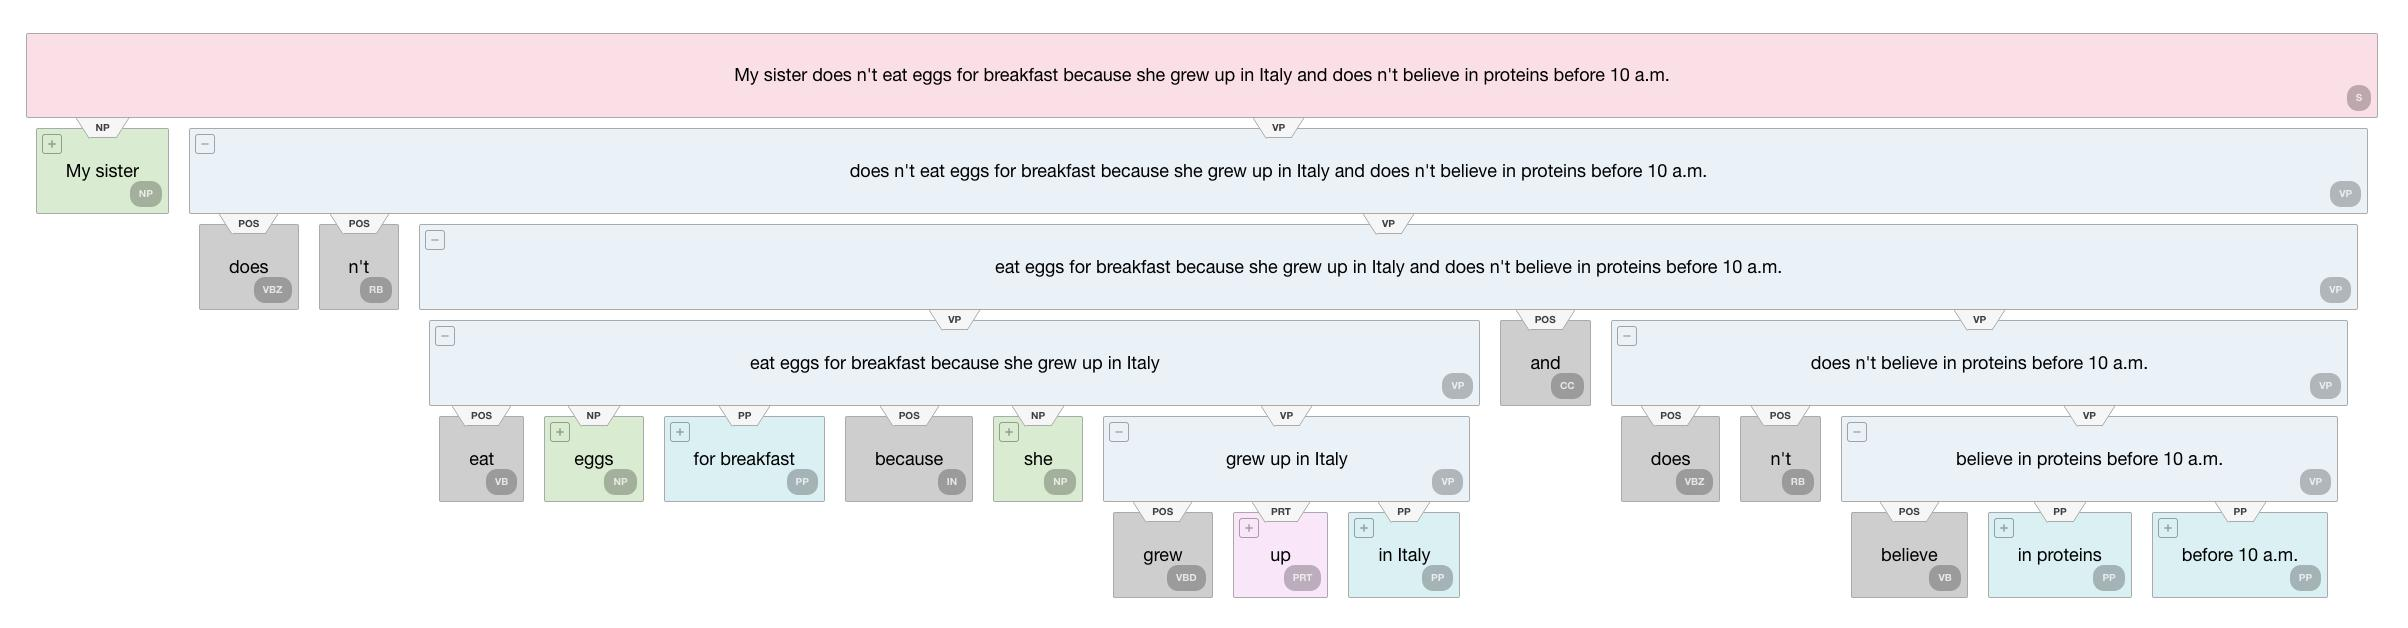
\includegraphics[width=\linewidth]{img/parse_tree_syntactic_parsing}
\end{center}

\subsubsection{Dependency Parsing}
Dependency Parsing helps in understanding what depends on what. The assumption is that the sentence is centred around the verb and what comes first in a sentence is more important than any information that comes after. So anything of the sentence depends on that word or some lower-level information.

\begin{center}
	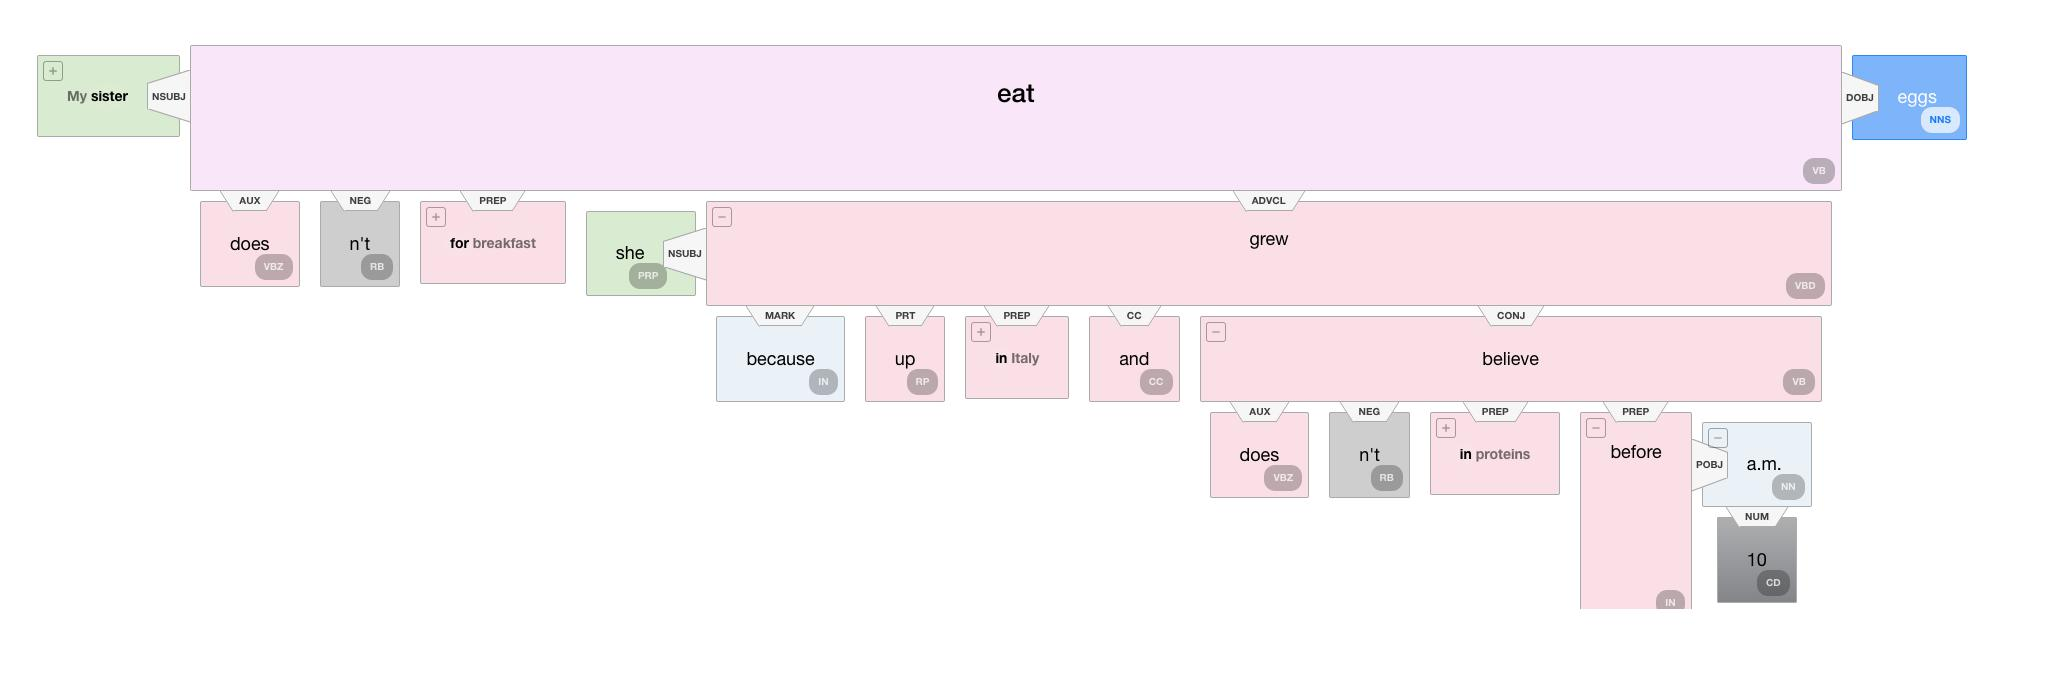
\includegraphics[width=\linewidth]{img/parse_tree_dependency_parsing}
\end{center}

\subsection{Understanding Meaning}
\subsubsection{Semantic Analysis}
\begin{itemize}
	\item word-level
	\begin{itemize}
		\item word sense disambiguation
		\item co-occurrence analysis
	\end{itemize}
	\item sentence-level or text-level
	\begin{itemize}
		\item semantic role labelling
		\item co-reference resolution
	\end{itemize}
\end{itemize}

\subsubsection{Discourse Analysis}
\begin{itemize}
	\item topics
	\item sentiments
	\item speech or dialogue acts
	\item argumentative structures
\end{itemize}

\subsection{Data for Text Analysis}
Text analysis using machine learning requires large amounts of training data and finding suitable data is often a bottleneck due to expense or limited rights. An annotated corpus typically contains a selection of texts based on explicit criteria, metadata like author, date, source, title, sectioning, and annotations in a more or less standardises format.

\subsection{Preprocessing}
Most text processing tasks begin with a set of standard preprocessing steps
\begin{itemize}
	\item Tokenisation: segmentation into tokens
	\item Token normalisation
	\item Segmentation into sentences
	\begin{center}
		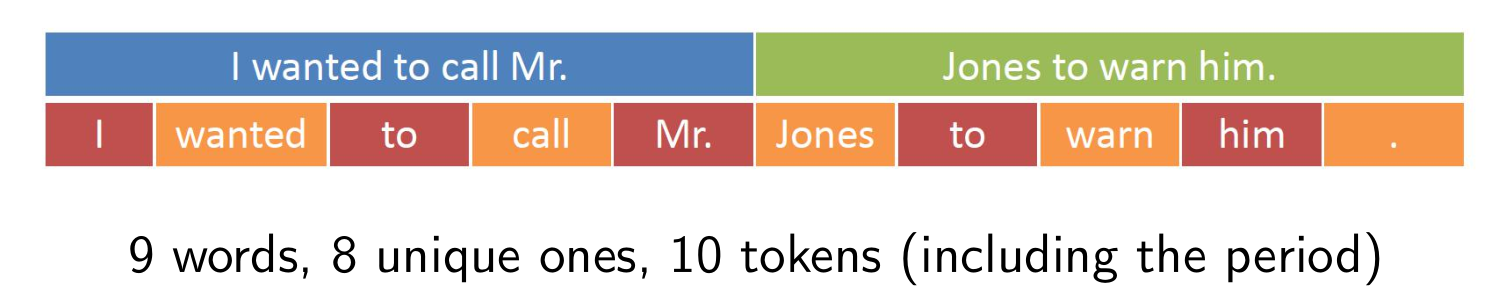
\includegraphics[width=0.8\linewidth]{img/sentence_segmentation}
	\end{center}
	\item There are about 170'000 unique words in the English language at the moment
\end{itemize}

\subsubsection{Tokens and Types}
Tokens are the words on the page, while the type is the word forms. Counting the types requires lemmatisation, which is finding the lemma or base form for each word.

\subsubsection{Tokenisation and Normalisation}
Not as straightforward as one may think
\begin{itemize}
	\item punctuation
	\begin{itemize}
		\item periods and commas appear within words or abbreviations
		\item special tokens in mail addresses or tweets
		\item apostrophes
	\end{itemize}
	\item capital letters
	\item compound words
	\begin{itemize}
		\item problem complicated without dashes
		\item German words
		\item proper names
	\end{itemize}
\end{itemize}

\subsubsection{Sentence Segmentation}
Can be easier or more difficult depending on the source text formatting. If no particular information is available from the layout, punctuations and casing can be used. While question and exclamation marks are quite reliable indicator of sentences periods are not. A good approach is to try to combine Tokenisation and Sentence Splitting, focusing on full stops.


\end{document}
